% ============================================================
% APPENDIX: Electrical engineering foundations
% ============================================================

\appendix
\renewcommand{\thesection}{\Alph{section}}
\setcounter{section}{0}

\section{Electrical engineering foundations}\label{sec:eefoundations}

This appendix collects the electrical physics underpinning the
reliability and hazard models of the main text. The goal is to make
explicit how power-system quantities — fault current, arc-flash
incident energy, harmonic distortion, generator transient response,
battery cell electrochemistry — translate into the parameters that
appear inside the actuarial hazard~\eqref{eq:hazard} and the
deterministic grace-period equation~\eqref{eq:tcrit}.

\subsection{Per-unit power system representation}\label{ss:pu}

Power system analysis is normally conducted in \emph{per unit} (p.u.)
quantities to handle multiple voltage levels uniformly. Given a base
power $S_{\mathrm{base}}$ (e.g.\ \SI{100}{\mega\volt\ampere}) and a
base voltage $V_{\mathrm{base}}$ at each level, derived bases are
\begin{equation}\label{eq:pu-bases}
   I_{\mathrm{base}} \;=\; \frac{S_{\mathrm{base}}}{\sqrt{3}\,V_{\mathrm{base}}},
   \qquad
   Z_{\mathrm{base}} \;=\; \frac{V_{\mathrm{base}}^2}{S_{\mathrm{base}}}.
\end{equation}
Any physical quantity $X$ becomes $X_{\mathrm{pu}}=X/X_{\mathrm{base}}$.
The voltage state $V_t$ in the SDE~\eqref{eq:sde} is dimensionless
precisely because it is a per-unit voltage measured at the LV bus, with
$V_t=1$ at nominal $V_{\mathrm{nom}}=\SI{480}{V}$.

\subsection{Symmetrical fault current and short-circuit power}\label{ss:fault}

Switchgear, breaker, transformer and conductor reliability are
governed by the prospective short-circuit current $I_{\mathrm{sc}}$ at
the fault location. For a three-phase symmetrical bolted fault, the
short-circuit current at a bus with Th\'evenin equivalent impedance
$Z_{\mathrm{th}}$ is
\begin{equation}\label{eq:Isc}
   I_{\mathrm{sc}} \;=\; \frac{V_{\mathrm{nom}}}{\sqrt{3}\,|Z_{\mathrm{th}}|},
   \qquad
   S_{\mathrm{sc}} \;=\; \sqrt{3}\,V_{\mathrm{nom}}\,I_{\mathrm{sc}}
   \;=\; \frac{V_{\mathrm{nom}}^2}{|Z_{\mathrm{th}}|},
\end{equation}
where $S_{\mathrm{sc}}$ is the short-circuit power. For a typical
\SI{2.5}{\mega\volt\ampere} step-down transformer with per-unit
impedance $z=0.0575$ feeding a \SI{480}{V} bus, the bus
$I_{\mathrm{sc}}$ is
\begin{equation}
   I_{\mathrm{sc}}
   \;=\; \frac{I_{\mathrm{base}}}{z}
   \;=\; \frac{1}{0.0575}\cdot\frac{2.5\times 10^6}{\sqrt{3}\cdot 480}
   \;\approx\; \SI{52}{\kilo\ampere}.
\end{equation}
This is the rms symmetrical component; the asymmetric peak in the
first half-cycle is approximately $2.7\,I_{\mathrm{sc}}\approx
\SI{140}{\kilo\ampere}$. The breaker interrupt rating must exceed
this value.

\subsection{Thévenin equivalent at the LV bus: schematic}\label{ss:thevenin}

Figure~\ref{fig:thevenin} shows the source-side impedance ``stack-up''
that determines $Z_{\mathrm{th}}$ in equation~\eqref{eq:Isc}: utility
source impedance, transformer impedance, and cable impedance combine
in series at the LV bus where the fault is calculated.

\begin{figure}[ht]
\centering
\begin{circuitikz}[american,
   scale=0.95,
   every node/.style={font=\footnotesize}]

% Utility source (Thevenin equivalent of the grid)
\draw (0,0) to[V,l_=$V_{\mathrm{grid}}$,invert] (0,2);
\draw (0,2) to[R,l=$R_g$] (2,2);
\draw (2,2) to[L,l=$jX_g$] (4,2);
\node at (4.5,2.6) {\scriptsize Utility};

% Transformer drawn as two adjacent inductors plus a divider
\draw (4,2) -- (5,2);
\draw (5,2) to[L,l=\,] (6.2,2);
\draw[ultra thick] (6.35,2.55) -- (6.35,1.45);
\draw[ultra thick] (6.55,2.55) -- (6.55,1.45);
\draw (6.7,2) to[L,l=\,] (7.9,2);
\node at (6.45,3.2) {\scriptsize TX 34.5/0.48\,kV};

% Transformer series impedance (lumped on LV side)
\draw (7.9,2) to[R,l=$R_T$] (9.4,2);
\draw (9.4,2) to[L,l=$jX_T$] (10.9,2);

% Cable
\draw (10.9,2) to[R,l=$R_c$] (12.2,2);
\draw (12.2,2) to[L,l=$jX_c$] (13.5,2);

% Fault location (LV bus)
\draw[thick,red] (13.5,2) -- (13.5,0.5);
\node[red] at (14.2,1.5) {\scriptsize fault $F$};
\draw[red,thick] (13.5,0.5) to[short,*-] (13.5,0.1);

% Ground return
\draw (13.5,-0.3) node[ground]{};
\draw (0,0) -- (13.5,0) -- (13.5,-0.1);

% Annotation
\node[align=left] at (6.5,-0.7)
  {\scriptsize $Z_{\mathrm{th}} = (R_g+R_T+R_c) + j(X_g+X_T+X_c)$};
\end{circuitikz}
\caption{Th\'evenin equivalent looking back from a fault point $F$ at
the LV bus. The total source-side impedance $Z_{\mathrm{th}}$
determines the prospective short-circuit current per
equation~\eqref{eq:Isc}. In a $2N$ data center, the same calculation
must be done assuming each path independently, and then for the
parallel combination, since closing the bus tie can dramatically
increase $I_{\mathrm{sc}}$.}
\label{fig:thevenin}
\end{figure}

\subsection{Arc-flash incident energy (IEEE~1584)}\label{ss:arcflash}

A bolted three-phase fault that ignites an electrical arc releases
enormous thermal energy in milliseconds. The IEEE~1584-2018 model
gives incident energy at working distance $D$ as
\begin{equation}\label{eq:arcflash}
   E \;=\; 4.184\, C_f\, E_n
   \left(\frac{t}{0.2}\right)\left(\frac{610^x}{D^x}\right)\quad
   \text{[J/cm$^2$]},
\end{equation}
where $E_n$ is the normalised incident energy, $C_f$ is a calculation
factor, $t$ is the arc duration (in seconds, governed by the
upstream protection clearing time), $D$ is the working distance
(typically \SI{457}{mm} for LV equipment), and $x$ is the
distance exponent ($\approx 1.5$ for open-air arcs in switchgear).

The protection clearing time $t$ is the critical lever: a properly
coordinated protective relay clears in $\sim\SI{50}{ms}$, giving
$E\sim\SI{5}{cal\per\cm\squared}$ (Category~2 PPE); a delayed clearing
of \SI{500}{ms} multiplies $E$ tenfold, into Category~4 ($>\SI{40}{cal
\per\cm\squared}$), the threshold above which survivable rescue of an
operator is essentially impossible and where a UPS-room fire becomes
a near-certainty. This is the deterministic origin of the
\emph{catastrophic} branch $F_{\mathrm{cat}}$ in the fault tree of
Figure~\ref{fig:fta}.

\begin{nbox}
\textbf{Underwriting implication.} Two otherwise-identical Tier-IV
sites can differ by $\sim 30\,\%$ in the catastrophic-loss tail
purely because of protective-relay coordination quality. The
arc-flash incident-energy survey, mandated annually by NFPA 70E for
US sites, is therefore a high-information underwriting document:
its category distribution across panels is a near-direct
estimator of the GPD shape parameter $\xi$ at that site.
\end{nbox}

\subsection{UPS double-conversion topology}\label{ss:ups}

Figure~\ref{fig:ups} is the canonical double-conversion (online) UPS:
the AC input passes through a rectifier ($\eta_{\mathrm{rec}}$) to a DC
bus, which both charges the battery string and feeds an inverter
($\eta_{\mathrm{inv}}$) producing a clean regulated AC output. In
this topology the load is permanently fed from the inverter, so the
transfer from utility-supported to battery-supported operation
involves \emph{no transient at the load}.

\begin{figure}[ht]
\centering
\begin{circuitikz}[american,
   scale=0.95,
   every node/.style={font=\footnotesize}]
% AC input
\draw (0,1) to[sV,l_=AC in] (0,3);
\draw (0,3) -- (1.5,3);

% Rectifier block
\draw (1.5,2.5) rectangle (3.3,3.5);
\node at (2.4,3) {\scriptsize Rectifier};
\node at (2.4,2.3) {\scriptsize $\eta_{\mathrm{rec}}$};

% DC bus
\draw (3.3,3) -- (5.0,3);
\draw[ultra thick,red] (5.0,2) -- (5.0,4);
\node[red] at (5.4,4.2) {\scriptsize DC bus};

% Battery string
\draw (5.0,2) -- (5.0,1.0);
\draw (4.7,1.0) -- (5.3,1.0);
\draw (4.5,0.7) -- (5.5,0.7);
\draw (4.7,0.4) -- (5.3,0.4);
\draw (4.5,0.1) -- (5.5,0.1);
\node at (6.4,0.55) {\scriptsize Li-ion string};
\node at (6.4,0.15) {\scriptsize $V_{\mathrm{batt}}\!\approx\!540\,$V};

% Inverter
\draw (5.0,3) -- (6.5,3);
\draw (6.5,2.5) rectangle (8.3,3.5);
\node at (7.4,3) {\scriptsize Inverter};
\node at (7.4,2.3) {\scriptsize $\eta_{\mathrm{inv}}$};

% AC out
\draw (8.3,3) -- (10,3);
\draw (10,3) to[short,-o] (10.3,3);
\node at (10.6,3.3) {\scriptsize AC out};

% Static bypass switch (around the converter)
\draw[blue,dashed] (1.5,3) -- (1.5,5);
\draw[blue,dashed] (1.5,5) -- (9.5,5);
\draw[blue,dashed] (9.5,5) -- (9.5,3);
\node[blue] at (5.5,5.3) {\scriptsize Static bypass switch};
\end{circuitikz}
\caption{Double-conversion (online) UPS topology. The rectifier and
inverter, each lossy at efficiency $\eta_{\mathrm{rec}},\eta_{\mathrm{inv}}\!\approx\!0.98$,
isolate the load from input disturbances. The blue dashed line is the
static bypass switch which closes within a half-cycle on inverter
failure. Total double-conversion efficiency
$\eta_{\mathrm{UPS}}=\eta_{\mathrm{rec}}\eta_{\mathrm{inv}}\approx 0.96$,
which is the dominant contributor to the PUE overhead.}
\label{fig:ups}
\end{figure}

\subsection{Battery cell electrochemistry: from Butler--Volmer to thermal runaway}\label{ss:battery}

The single most consequential physical mechanism in modern data center
fires is lithium-ion thermal runaway. We sketch the underlying
electrochemistry to motivate the critical-boundary temperature
$T^*$ in Definition~\ref{def:hit}.

The current density $i$ across a battery electrode is given by the
Butler--Volmer equation
\begin{equation}\label{eq:BV}
   i \;=\; i_0\left[
   \exp\!\left(\frac{\alpha_a F\,\eta}{R\,T}\right)
   - \exp\!\left(-\frac{\alpha_c F\,\eta}{R\,T}\right)\right],
\end{equation}
with exchange current density $i_0$, charge transfer coefficients
$\alpha_a,\alpha_c$, Faraday constant $F$, overpotential $\eta$, gas
constant $R$, and absolute temperature $T$. Total heat generation
per cell, summed across reversible (entropic), irreversible (ohmic
and polarization) and side-reaction contributions, is
\begin{equation}\label{eq:Qcell}
   \dot Q_{\mathrm{cell}} \;=\;
   I(V_{\mathrm{oc}} - V) \;+\; I\,T\,\frac{\partial V_{\mathrm{oc}}}{\partial T}
   \;+\; \dot Q_{\mathrm{side}},
\end{equation}
where $V_{\mathrm{oc}}$ is open-circuit voltage and $V$ terminal
voltage. The first two are normal-operation terms; $\dot Q_{\mathrm{side}}$
captures decomposition reactions (SEI breakdown above $\sim\SI{80}{\celsius}$,
electrolyte decomposition above $\sim\SI{120}{\celsius}$, separator
melt $\sim\SI{135}{\celsius}$, cathode decomposition above
$\sim\SI{200}{\celsius}$) that become self-sustaining once they
start.

Coupling~\eqref{eq:Qcell} with a single-node thermal model gives the
classic \emph{Semenov} criterion for thermal runaway:
\begin{equation}\label{eq:semenov}
   \boxed{\;
   \frac{\dd \dot Q_{\mathrm{side}}}{\dd T} \;>\; h A,
   \;}
\end{equation}
where $hA$ is the cell's heat-rejection conductance (convection+radiation+conduction
to neighbours). The temperature at which the inequality first holds is
the critical boundary $T^*$ of equation~\eqref{eq:hitting}. For
NMC-622 cells at typical pack densities, $T^*\approx\SI{135}{\celsius}$,
i.e.\ a temperature rise above ambient room temperature of
$\Delta T\approx\SI{110}{\kelvin}$ --- but for off-gas vented cells in
a dense rack arrangement the effective $T^*$ can be as low as
$\sim\SI{60}{\celsius}$ due to mutual heating.

\begin{rbox}
The Semenov boundary~\eqref{eq:semenov} is what off-gas detection
moves: by triggering ventilation and isolation \emph{before} a single
cell vents into its neighbours, $hA$ is effectively raised
(forced convection added) so $T^*$ shifts upward, restoring margin.
This is the physical mechanism behind the 40--60\% loss-cost
reduction claimed for off-gas retrofits in the main text.
\end{rbox}

\subsection{Power quality: sags, harmonics, total harmonic distortion}\label{ss:pq}

The voltage state $V_t$ in the SDE \eqref{eq:sde} is a scalar
abstraction of a much richer reality. For balanced three-phase AC
the instantaneous waveform admits a Fourier representation
\begin{equation}\label{eq:fourier}
   v(t) \;=\; \sum_{n=1}^{\infty} V_n\,\sin(n\omega_0 t + \phi_n),
   \qquad \omega_0 = 2\pi f_0,
\end{equation}
with $f_0=\SI{50}{\hertz}$ or \SI{60}{\hertz}. The total harmonic
distortion (THD) of voltage is
\begin{equation}\label{eq:THD}
   \mathrm{THD}_V \;=\;
   \frac{\sqrt{\sum_{n=2}^{\infty} V_n^2}}{V_1}.
\end{equation}
IEEE~519 requires $\mathrm{THD}_V<5\%$ at the point of common
coupling. AI-training workloads, with their sub-millisecond GPU power
swings, push large dynamic currents through the UPS inverters and can
elevate $\mathrm{THD}_I$ above $15\%$, causing transformer derating
($K$-factor) and accelerated insulation ageing. This is the
mechanistic origin of the voltage-stress exponent $\gamma_V$ in the
hazard~\eqref{eq:hazard}: under accelerated insulation ageing models,
\begin{equation}\label{eq:AIPL}
   \mathrm{Life}(V,T) \;=\;
   A\cdot V^{-\gamma_V}\cdot\exp\!\left(\frac{E_a}{k_B T}\right),
\end{equation}
which is the Arrhenius--inverse-power-law (AIPL) model. The
$\gamma_V\in[3,7]$ range cited in \S\ref{sec:coupled} comes
directly from~\eqref{eq:AIPL} fitted to liquid-filled-transformer
endurance data.

\paragraph{Voltage sags.} A voltage sag is a momentary RMS reduction
to \mbox{0.1--0.9}\,p.u.\ for half a cycle to one minute. The
ITIC/CBEMA curve (Figure~\ref{fig:itic}) defines tolerance envelopes;
sags falling below the lower curve trip the UPS to battery. Sag
occurrence rate at the LV bus is empirically Poisson with intensity
5--30 events/year for utility feeds, dominated by upstream faults on
the distribution system. This populates the jump term
$J^V_t\,\dd N^V_t$ in~\eqref{eq:sde}.

\begin{figure}[ht]
\centering
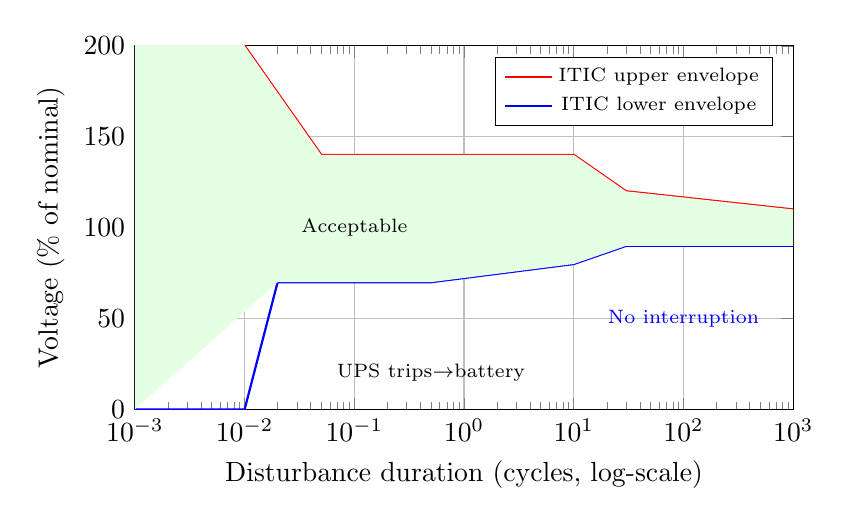
\begin{tikzpicture}
\begin{semilogxaxis}[
  width=0.82\linewidth, height=6.2cm,
  xlabel={Disturbance duration (cycles, log-scale)},
  ylabel={Voltage (\%\ of nominal)},
  xmin=0.001, xmax=1000, ymin=0, ymax=200,
  grid=major,
  legend pos=north east,
  legend style={font=\scriptsize},
  log basis x=10,
]
% Upper envelope (overvoltage tolerance)
\addplot[red,thick] coordinates {
  (0.001,500) (0.01,200) (0.05,140) (0.5,140)
  (10,140) (30,120) (1000,110) };
\addlegendentry{ITIC upper envelope}

% Lower envelope (undervoltage tolerance)
\addplot[blue,thick] coordinates {
  (0.001,0) (0.01,0) (0.02,70) (0.5,70)
  (10,80)  (30,90)  (1000,90) };
\addlegendentry{ITIC lower envelope}

% Acceptable region shading
\addplot[fill=green!10,draw=none,forget plot] coordinates
  { (0.02,70) (0.5,70) (10,80) (30,90) (1000,90) (1000,110)
    (30,120) (10,140) (0.5,140) (0.05,140) (0.01,200) (0.001,500)
    (0.001,0) (0.02,70) };

% Annotations
\node[font=\scriptsize] at (axis cs:0.1,100) {Acceptable};
\node[font=\scriptsize,red] at (axis cs:0.005,300) {No damage};
\node[font=\scriptsize,blue] at (axis cs:100,50) {No interruption};
\node[font=\scriptsize] at (axis cs:0.5,20)  {UPS trips$\to$battery};
\end{semilogxaxis}
\end{tikzpicture}
\caption{Stylised ITIC/CBEMA voltage tolerance envelope. The
green band is the safe operating region for sensitive IT equipment.
Excursions below the lower (blue) curve cause the UPS to drop the
load to battery; excursions above the upper (red) curve risk
damage to power supply units. The horizontal axis is logarithmic in
cycles at \SI{50}{\hertz}/\SI{60}{\hertz}, spanning roughly half a
microsecond to 20 seconds.}
\label{fig:itic}
\end{figure}

\subsection{Generator transient response and the ATS transfer window}\label{ss:atw}

When utility power fails, the Automatic Transfer Switch (ATS) signals
the standby generator to start. The diesel/gas engine accelerates,
the alternator field is excited, and once voltage and frequency are
within tolerance the ATS closes onto the generator. The full
sequence takes 8--12 seconds, but the most violent part is the
\emph{first cycle} of loading.

The generator's transient response when loaded is governed by its
sub-transient reactance $X_d''$, transient reactance $X_d'$, and
synchronous reactance $X_d$:
\begin{equation}\label{eq:Igen}
   I(t) \;=\; E_f \left[
   \frac{1}{X_d} + \left(\frac{1}{X_d'}-\frac{1}{X_d}\right)e^{-t/T_d'}
            + \left(\frac{1}{X_d''}-\frac{1}{X_d'}\right)e^{-t/T_d''}\,\right],
\end{equation}
where $T_d', T_d''$ are the corresponding time constants
(seconds, milliseconds respectively) and $E_f$ is field voltage.
Equation~\eqref{eq:Igen} explains why the load step that the generator
sees in its first second is several times the steady-state current:
the sub-transient reactance is much smaller than the synchronous, so
the initial current spike is large. Conservative generator sizing
($\geq 125\%$ of nominal IT load) is a direct response to this transient.

\subsection{Earthing scheme and fault propagation}\label{ss:earth}

The way the neutral is referenced to earth determines how a phase-to-earth
fault behaves --- whether it appears as a small leakage current that an
RCD detects, or as a near-bolted-fault that triggers main breaker action.

Three schemes are common:
\begin{itemize}[leftmargin=*,nosep]
  \item \textbf{TN-S} (separate neutral and protective earth):
        first phase-to-earth fault is a full short circuit, cleared by
        the breaker. Dominant in IT/PDU layers because it gives
        predictable short-circuit currents.
  \item \textbf{TN-C-S}: combined upstream, separated downstream;
        good cost-performance tradeoff but vulnerable to PEN-conductor breaks.
  \item \textbf{IT} (isolated neutral): first earth fault gives only a
        small displacement current; the second fault, on a different
        phase, becomes a phase-to-phase short. Used in some EU sites
        for continuity-of-service but requires insulation monitoring.
\end{itemize}
The choice affects how the elementary events $E_\bullet$ in the
fault tree~\eqref{eq:topdown} compose: in an IT scheme, the first-fault
event is harmless but the second-fault event is large; the joint
distribution is therefore highly non-Markovian and an additional state
must be added to the chain of Figure~\ref{fig:markov}.

\subsection{Putting the physics back into the hazard}\label{ss:closure}

We can now interpret each term of the hazard rate
\eqref{eq:hazard} in physical units:
\begin{equation*}
   \lambda_t \;=\; \lambda_0\, e^{-E_a/k_B T_t}
              \cdot \bigl(V_t/V_{\mathrm{nom}}\bigr)^{-\gamma_V}
              \cdot \exp(\beta_C C_t).
\end{equation*}
\begin{itemize}[leftmargin=*,nosep]
  \item $\lambda_0$ has dimensions of $\mathrm{events}/\mathrm{year}$,
        and is obtained from the steady-state Markov-chain analysis
        of \S\ref{ss:markov} together with the Th\'evenin/short-circuit
        analysis of \S\ref{ss:fault}.
  \item $E_a$ is the AIPL activation energy of the insulation system
        (transformer paper, capacitor dielectrics), \SI{0.6}{}--\SI{0.9}{\electronvolt}.
  \item $\gamma_V$ is the inverse-power-law voltage stress exponent
        from~\eqref{eq:AIPL}, calibrated from THD measurements
        \eqref{eq:THD} and dielectric endurance tests.
  \item $\beta_C C_t$ is the cyber-load Esscher tilt, with $C_t$
        in standardised log-rate units.
\end{itemize}
The deterministic grace period~\eqref{eq:tcrit} contains $UA$ and
$mc_p$, which an EE/HVAC engineer measures directly during
commissioning. \emph{This is the closure of the loop}: every parameter
in the actuarial pricing equation has a physical measurement
attached, and the parameters are identified, not assumed.
